\begin{note}
    此小节还未完成。
\end{note}

\subsection{滤波器的表示}

\subsubsection{什么是滤波器}

\begin{definition}
    \bd{滤波器}是以特定方式改变信号的频率特性,从而变换信号的处理系统。
    滤波器一般有如下类别,如图 \ref{fig:filter-types} 所示:
    \begin{enumerate}[label=(\arabic*)]
        \item 高通滤波器(HP)
        \item 低通滤波器(LP)
        \item 带通滤波器(BP)
        \item 带阻滤波器(BS)
        \item 全通滤波器(AP)
    \end{enumerate}
    \begin{figure}[H]
        \centering
        \includegraphics[width=0.8\textwidth]{chap4/img/filter_types.png}
        \caption{滤波器类型}
        \label{fig:filter-types}
    \end{figure}

    滤波器也可以被分为\bd{模拟滤波器}和\bd{数字滤波器}。
    \begin{itemize}
        \item \bd{模拟滤波器}是由电阻、电容、电感等部件构成的电路。
            滤波器特性对所用部件的物理标称值非常敏感,而且,
            有些部件的物理特性会随温度变化而改变。
        \item \bd{数字滤波器}是用软件实现的,很少依赖硬件。滤波软件
            只是一系列程序指令。虽然它是在硬件平台上运行,但
            是硬件平台本身并不决定滤波器的性能。数字滤波器的
            性能是由\bd{一组系数}确定的。
    \end{itemize}
    数字滤波器的实现方式一般有以下几种:
    \begin{enumerate}
        \item 用流图计算滤波器的输出。
        \item 用差分方程计算滤波器的输出。
        \item 用卷积过程计算滤波器的输出。
        \item 用 DTFT 直接改变信号频谱。
    \end{enumerate}
\end{definition}

\begin{property}[滤波器的滤波特性参数]
    (低通)滤波器的滤波特性参数如图 \ref{fig:filter-characteristics} 所示。
    虚线表示的是\bd{理想低通滤波器}的滤波特性,实线表示的是\bd{窗函数法}设计
    得到的\bd{实际低通滤波器}的滤波特性。
    \begin{figure}[H]
        \centering
        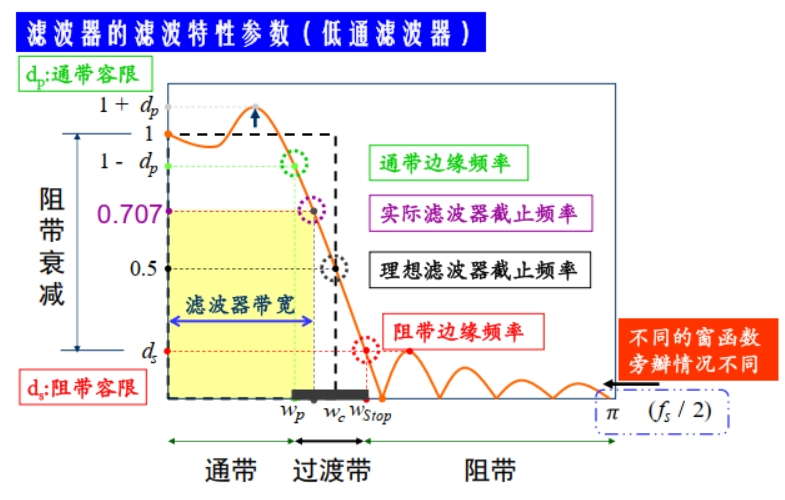
\includegraphics[width=0.8\textwidth]{chap4/img/filter_characteristics.png}
        \caption{滤波器的滤波特性参数}
        \label{fig:filter-characteristics}
    \end{figure}
\end{property}

\subsubsection{什么是系统}

滤波器是以特定方式改变信号的频率特性的系统。那么,什么是系统呢?

\begin{definition}[系统]
    \bd{系统}是由若干相互作用和相互依赖的事物组合而成的具有特定功能的整体。例如,
    计算机系统、医疗系统、雷达导航系统等。

    通俗地说,对信号处理的各种环境都可以被称为系统。在信号处理领域,系统是为了
    传送信号或对信号进行加工处理而构成的某种组合。这种组合,既可以有对应的物理设备,
    如电容、放大器等,也可以是纯粹的算法,如计算机软件程序等;关键在于,系统是
    一个具有``特定功能的整体''。
\end{definition}

\subsubsection{系统的分类}

\begin{definition}[连续时间系统与离散时间系统]
    系统可以分为连续时间系统和离散时间系统。
    \begin{itemize}
        \item \bd{连续时间系统}是指输入和输出的信号都是连续时间信号,
            并且在系统内部也没有对信号进行转换的系统。
        \item \bd{离散时间系统}是指输入和输出的信号都是离散时间信号,
            并且在系统内部,信号也是离散时间的形式的系统。
    \end{itemize}
    
    对于这两种不同的系统类别,它们的系统原理和分析方法,除少部分内容不同外,
    其余大部分内容是相同的。本章主要讨论离散时间系统。
\end{definition}

\begin{definition}[线性系统]
    同时满足叠加性与齐次性的系统称为\bd{线性系统}。
    \begin{itemize}
        \item 满足\bd{叠加性}是指:当几个输入信号同时输入系统时,系统总的
            输出等于几个输入信号单独输入系统时的输出信号和。
        \item 满足\bd{齐次性}是指:当输入信号乘以某个常数时,系统的输出也
            乘以相同的常数。
    \end{itemize}
\end{definition}

\begin{definition}[时不变系统]
    若系统既是线性的,又是时不变的,则称其为\bd{线性时不变系统},简称\bd{LTI 系统}。
\end{definition}

\begin{definition}[因果系统]
    如果系统的输出取决于现在和以前的输入数据,而与以后的输入数据无关,
    则称该系统为\bd{因果系统}。所有实际系统都是因果系统。
\end{definition}

\begin{definition}[稳定系统]
    若系统在有界输入下产生有界输出,则称该系统为\bd{稳定系统}。
    这个性质通常被称为 \bd{BIBO(Bounded Input, Bounded Output) 原则}。
\end{definition}

\begin{remark}
    为什么要研究滤波器这一系统呢?
    因为我们需要对信号进行处理,而滤波器是信号处理的重要工具。
    \begin{itemize}
        \item 对于具有特定参数的系统,它具有何种处理信号的特性?
            \subitem 即:分析信号在通过系统后,信号的特性会发生怎样的变化?
        \item 对于给定的传输和处理信号的要求,如何设计并实现一个与其相匹配的系统?
            \subitem 即:如何设计并实现系统,使系统满足信号处理的要求?系统应具有怎样的功能和参数?
    \end{itemize}
\end{remark}

\subsubsection{用差分方程表示系统}

\label{subsubsection:diff-equation-representation}

\begin{definition}[差分方程]
    \bd{差分方程}是描述离散时间系统的一种数学模型。对于线性时不变系统,
    差分方程的一般形式为
    \begin{align*}
        \sum_{k = 0}^{N}b(k)y(n - k) = \sum_{k = 0}^{M}a(k)x(n - k).
    \end{align*}
    其中,$x(n)$ 是输入信号,$y(n)$ 是输出信号,$a(k), b(k)$ 是系统的系数。$N$ 为
    所需过去输出的个数,通常称为滤波器的\bd{阶数}。
\end{definition}

\begin{example}
    如下是一个差分方程的例子:
    \begin{align*}
        y(n) = \frac{1}{b_0}(a_0x(n) + a_1x(n - 1) - b_1(y(n - 1))).
    \end{align*}
\end{example}

\subsubsection{用流图表示系统}

\label{subsubsection:flow-chart-representation}

\begin{definition}[流图]
    \bd{流图}是描述系统的输入输出关系的图形表示法。流图中,用方框表示系统,
    用箭头表示信号的流动方向。流图的优点是直观,易于理解。

    以下是流图中常见的符号:
    \begin{itemize}
        \item 延时单元

    \end{itemize}
\end{definition}

\begin{exercise}
    画出下列差分方程对应的流图:
    \begin{align*}
        y(n) = \frac{1}{b_0}(a_0x(n) + a_1x(n - 1) - b_1(y(n - 1))).
    \end{align*}
\end{exercise}

\begin{solution}
    该差分方程对应的流图如图 \ref{fig:chap4-part1-quiz1} 所示。
    \begin{figure}[H]
        \centering
        \tikzstyle{block} = [draw, rectangle, minimum height=1cm, minimum width=1cm]
        \tikzstyle{circ} = [draw, fill, circle, inner sep=1.5pt]
        \tikzstyle{no-circ} = [draw, circle, inner sep=0pt]
        \tikzstyle{sum} = [draw, circle]
        \tikzstyle{line} = [draw, -latex]
        \tikzstyle{no-arrow-line} = [draw, -]
        \tikzstyle{gainx} = [draw, isosceles triangle, isosceles triangle apex angle=60]
        \tikzstyle{gainy} = [draw, isosceles triangle, isosceles triangle apex angle=60, shape border rotate=180]
        \begin{tikzpicture}
            \node [name=input] (input) {$x(n)$};
            \node [circ, right of=input, xshift=1cm] (circx) {};
            \path [no-arrow-line] (input) -- (circx);
            \node [sum, right of=circx, xshift=4cm] (sum) {$+$};
            \node [circ, right of=sum, xshift=4cm] (circy) {};
            \node [name=output, right of=circy, xshift=1cm] (output) {$y(n)$};
            \path [line] (circy) -- (output);
    
            \node [block, below of=circx, yshift=-1cm] (zx1) {$Z^{-1}$};
            \path [line] (circx) -- (zx1);
    
            \node [block, below of=circy, yshift=-1cm] (zy1) {$Z^{-1}$};
            \path [line] (circy) -- (zy1);
    
            \node [gainx, right of=circx, xshift=1cm] (zgx0) {$a_0$};
            \path [line] (circx) -- (zgx0);
            \path [line] (zgx0) -- (sum);
            \node [gainx, below of=zx1, xshift=2cm, yshift=-0.5cm] (zgx1) {$a_1$};
            \path [line] (zx1) |- (zgx1);
            \path [line] (zgx1.east) -- (sum);
            \node [gainx, right of=sum, xshift=2cm] (zgy0) {$1/b_0$};
            \path [line] (sum) -- (zgy0);
            \path [line] (zgy0) -- (circy);
            \node [gainy, below of=zy1, xshift=-2cm, yshift=-0.5cm] (zgy1) {$-b_1$};
            \path [line] (zy1) |- (zgy1);
            \path [line] (zgy1.west) -- (sum);
        \end{tikzpicture}
        \caption{习题 \theexercise~ 信号流图}
        \label{fig:chap4-part1-quiz1}
    \end{figure}
\end{solution}

\subsubsection{零输入响应与零状态响应}

常见的两种系统响应是\bd{零输入响应}和\bd{零状态响应}。

\begin{definition}[零输入响应]
    系统可能在没有给任何激励信号作用时,产生信号输出。
    在这种情况下,系统的输出显然是与外界无关的(因为外界并没有给系统输入信号),
    输出是由系统自身的内部信息引起的。

    系统自身的内部信息,可能是先前激励(或挠动)作用的后果;
    不过,没有必要追究它们历史演变的详细过程,只需知道在当前激励接入系统时,
    系统瞬时状态即可。

    由此看来,系统的零输入响应是一种纯粹由系统的起始状态所产生的响应。
\end{definition}

\begin{definition}[零状态响应]
    系统在每一时刻都对应一种状态,开始研究系统的时刻系统所处的状态称为起始状态。
    所谓系统的零状态响应,就是指系统在起始状态时状态值为零(相当于系统没有存储任何能量和信息)。

    在这种状况下,给系统输入一个激励信号,则系统所产生输出响应就被称为系统的零状态响应。
\end{definition}

\begin{definition}[滤波器的脉冲响应(冲激响应)]
    \bd{滤波器的脉冲响应}(冲激响应)是指滤波器对脉冲输入的响应,
    即:当滤波器的输入为单位脉冲信号 $\delta(n)$ 时,滤波器的输出为单位脉冲响应。
\end{definition}

\begin{remark}
    系统的输入输出关系可以由图 \ref{fig:system-input-output} 总结。
    \begin{figure}[H]
        \centering
        \begin{tikzpicture}
            \node (input) [draw, rectangle, minimum width=2cm, minimum height=1cm] at (0, 0) {输入信号(激励)};
            \node (system) [draw, rectangle, minimum width=2cm, minimum height=1cm] at (5, 0) {系统};
            \node (output) [draw, rectangle, minimum width=2cm, minimum height=1cm] at (10, 0) {输出信号(响应)};
        
            \draw[->] (input) --  (system);
            \draw[->] (system) -- (output);
        \end{tikzpicture}
        \caption{系统的输入输出关系}
        \label{fig:system-input-output}
    \end{figure}
\end{remark}

\begin{example}
    求下列滤波器脉冲响应的前六个采样值:
    \begin{align*}
        y(n) = 0.25(x(n) + x(n - 1) + x(n - 2) + x(n - 3))
    \end{align*}
\end{example}

\begin{solution}
    用 $\delta(n)$ 代替 $x(n)$,用 $h(n)$ 代替 $y(n)$,则有
    \begin{align*}
        h(n) = 0.25(\delta(n) + \delta(n - 1) + \delta(n - 2) + \delta(n - 3)).
    \end{align*}

    由此可得 $h(n)$ 的前六个采样值为
    \begin{align*}
        h(0) & = 0.25, \\
        h(1) & = 0.25, \\
        h(2) & = 0.25, \\
        h(3) & = 0.25, \\
        h(4) & = 0, \\
        h(5) & = 0.
    \end{align*}
\end{solution}

\begin{exercise}
    求下列滤波器脉冲响应的前六个采样值,其中滤波器是因果系统(即,脉冲响应在 $n < 0$ 时为零):
    \begin{align*}
        y(n) - 0.4y(n - 1) = x(n) - x(n - 1).
    \end{align*}
\end{exercise}

\begin{solution}
    用 $\delta(n)$ 代替 $x(n)$,用 $h(n)$ 代替 $y(n)$,则有
    \begin{align*}
        h(n) - 0.4h(n - 1) = \delta(n) - \delta(n - 1).
    \end{align*}

    由于该滤波器为因果系统,故 $h(-1) = 0$。由此可得 $h(n)$ 的前六个采样值为
    \begin{align*}
        h(0) & = 1, \\
        h(1) & = -0.6, \\
        h(2) & = -0.24, \\
        h(3) & = -0.096, \\
        h(4) & = -0.0384, \\
        h(5) & = -0.01536.
    \end{align*}
\end{solution}

\subsubsection{FIR 和 IIR 滤波器}

\begin{example}
    \label{exercise:serial-flow-chart}
    写出如图 \ref{fig:serial-flow-chart} 所示级联流图的差分方程。
    \begin{figure}[H]
        \centering
        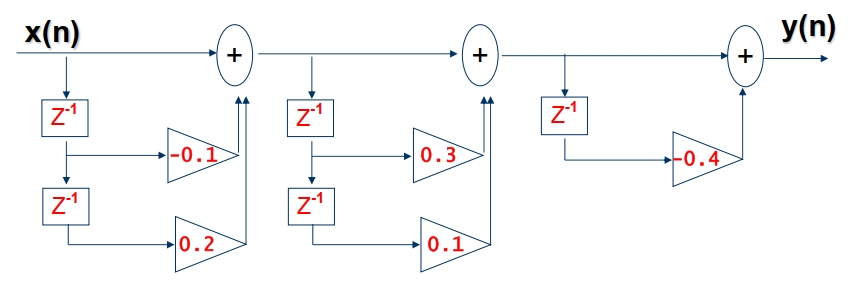
\includegraphics[width=0.8\textwidth]{chap4/img/serial_flow_chart.png}
        \caption{例 \theexample~ 的级联流图}
        \label{fig:serial-flow-chart}
    \end{figure}
\end{example}

\begin{solution}
    不妨设 $x(n) = x_1(n), y(n) = y_3(n)$,
    以及 $y_1(n) = x_2(n), y_2(n) = x_3(n)$,则如图 \ref{fig:serial-flow-chart-annotated} 所示,
    \begin{align*}
        y_1(n) & = x_1(n) - 0.1x_1(n - 1) + 0.2x_1(n - 2), \\
        y_2(n) & = x_2(n) + 0.3x_2(n - 1) + 0.1x_2(n - 2), \\
        y_3(n) & = x_3(n) - 0.4x_3(n - 1).
    \end{align*}
    \begin{figure}[H]
        \centering
        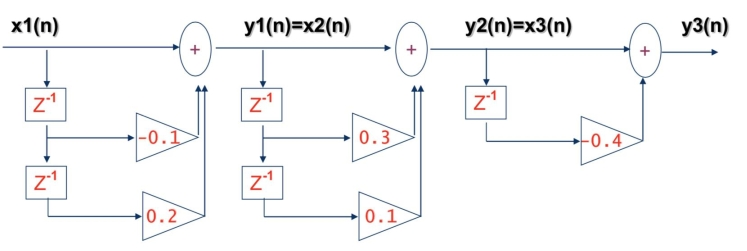
\includegraphics[width=0.8\textwidth]{chap4/img/serial_flow_chart_annotated.png}
        \caption{例 \theexample~ 的级联流图(带标注)}
        \label{fig:serial-flow-chart-annotated}
    \end{figure}
    将 $y_1(n)$ 代入 $y_2(n)$ 的表达式中,将 $y_2(n)$ 代入 $y_3(n)$ 的表达式中,
    可得级联流图的差分方程为
    \begin{align*}
        y_3(n) = x_1(n) - 0.2x_1(n - 1) + 0.19x_1(n - 2) - 0.058x_1(n - 3) - 0.008x_1(n - 5).
    \end{align*}
\end{solution}

\subsubsection{用脉冲响应表示系统}

\label{subsubsection:pulse-response-representation}

\begin{theorem}
    设某滤波器的脉冲响应为 $h(n)$,某输入信号为 $x(n)$。则输入信号可以表示
    为一系列脉冲函数之和:
    \begin{align*}
        x(n) = \sum_{k = -\infty}^{+\infty}x(k)\delta(n - k).
    \end{align*}
    当输入单位脉冲时,即 $x(n) = \delta(n)$,滤波器的输出响应为 $h(n)$,
    则根据 LTI 系统的线性性质和时不变性特性,输入 $x(n)$ 时的输出为
    \begin{align*}
        y(n) = \sum_{k = -\infty}^{+\infty}x(k)h(n - k) = x(n) * h(n).
    \end{align*}
    
    即,\bd{数字滤波器的输出等于输入信号,与脉冲响应的卷积}。
\end{theorem}

\begin{property}[差分方程与卷积运算]
    \label{property:diff-equation-convolution}
    写出 FIR 和 IIR 系统的差分方程如下:
    \begin{align*}
        \sum_{k = 0}^{N}b(k)y(n - k) & = \sum_{k = 0}^{M}a(k)x(n - k) \qquad \text{(IIR)} \\
        y(n) & = \sum_{k = 0}^{M}a(k)x(n - k) \qquad \text{(FIR)}
    \end{align*}
    在 FIR 系统的差分方程中,实际上系数 $a(k)$ 就是系统的脉冲响应 $h(k)$。也就是说,有
    \begin{align*}
        y(n) = a(n) * x(n) \qquad \text{(FIR)}
    \end{align*}

    卷积和差分方程都可以用来计算滤波器的输出。对于 FIR 而言,卷积运算和差分方程都适用;
    对于 IIR 而言,差分方程更加方便。
\end{property}

\begin{remark}
    由以上讨论可知,描述系统的方式有以下几种:
    \begin{itemize}
        \item 系统的差分方程,见 \ref{subsubsection:diff-equation-representation} 节。
        \item 流图,见 \ref{subsubsection:flow-chart-representation} 节。
        \item 数字系统的脉冲响应 $h(n)$,见 \ref{subsubsection:pulse-response-representation} 节。
    \end{itemize}
\end{remark}

\begin{exercise}
    \label{exercise:LTI-stable}
    证明:某 LTI 系统稳定的充要条件是
    \begin{align*}
        \sum_{n = -\infty}^{\infty} \abs{h(n)} = P < \infty.
    \end{align*}
    其中 $h(n)$ 为系统的单位脉冲响应,$P$ 为一个常数。
\end{exercise}

\begin{proof}
    首先证明必要性。不妨设 $\sum_{n= -\infty}^{+\infty}\abs{h(n)} = A$,
    对任意的有界输入 $x(n)$,设 $\forall n, \abs{x(n)} < B$。则
    \begin{align*}
        \abs{y(n)} & = \abs{x(n) * h(n)} = \abs{\sum_{k = -\infty}^{+\infty}h(k)x(n - k)} \\
        & \le \sum_{k = -\infty}^{+\infty} \abs{h(k)} \cdot \abs{x(n - k)} \\
        & < B \sum_{k = -\infty}^{+\infty} \abs{h(k)} = AB
    \end{align*}
    也有界。

    接下来证明充分性。使用反证法,设 $\sum_{n = -\infty}^{\infty} \abs{h(n)}$ 发散时,系统稳定。
    考虑输入
    \begin{align*}
        x(n) = \begin{cases}
                0, & h(-n) = 0, \\
                \sgn{h(-n)}, & h(-n) \neq 0.
            \end{cases}
    \end{align*}
    显然输入是有界的,且 $\forall n, \abs{x(n)} \le 1$。而
    \begin{align*}
        y(0) & = (x * h)(0) = \sum_{k = -\infty}^{+\infty}h(k)x(-k) \\
        & = \sum_{k = -\infty}^{+\infty}h(k) \cdot \sgn{h(k)} \\
        & = \sum_{k = -\infty}^{+\infty}\abs{h(k)}
    \end{align*}
    这个结果发散,说明输出是无界的,这与系统稳定相矛盾。故假设不成立,
    也就是说 $\sum_{n = -\infty}^{\infty} \abs{h(n)}$ 是收敛的。

    命题得证。
\end{proof}

\begin{property}[系统的串、并联组合]
    \label{property:parallel-serial-system}
    系统在串联和并联的情况下,其传递函数的组合规律如下:
    \begin{itemize}
        \item 两个系统的\bd{并联}后新系统的单位冲激响应是并联子系统的单位冲激响应之和,
            传递函数是并联子系统的传递函数之和。如图 \ref{fig:parallel-system} 所示,
            是一个并联系统。
            \begin{align*}
                h(n) = h_1(n) + h_2(n), \quad H(z) = H_1(z) + H_2(z).
            \end{align*}
        \item 两个系统的\bd{串联}后新系统的单位冲激响应是串联子系统的单位冲激响应的卷积,
            传递函数是串联子系统的传递函数的乘积。如图 \ref{fig:serial-system} 所示,
            是一个串联系统。
            \begin{align*}
                h(n) = h_1(n) * h_2(n), \quad H(z) = H_1(z) \cdot H_2(z).
            \end{align*}
    \end{itemize}
    \begin{figure}[H]
        \centering
        \begin{subfigure}{0.45\textwidth}
            \centering
            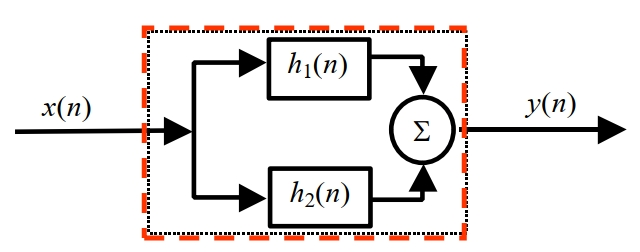
\includegraphics[width=\textwidth]{chap4/img/parallel_system.png}
            \caption{并联系统}
            \label{fig:parallel-system}
        \end{subfigure}
        \begin{subfigure}{0.45\textwidth}
            \centering
            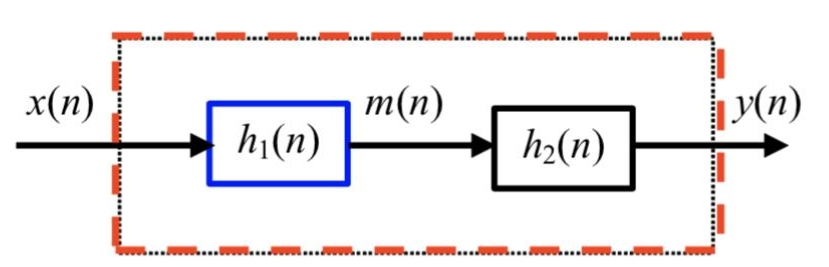
\includegraphics[width=\textwidth]{chap4/img/serial_system.png}
            \caption{串联系统}
            \label{fig:serial-system}
        \end{subfigure}
        \caption{系统的串、并联组合}
    \end{figure}
\end{property}

\subsubsection{系统的频率响应}

\begin{definition}[系统的频率响应]
    \bd{系统的频率响应},简称\bd{频响},反映了系统对激励中各频率分量的幅度和相位的影响。
    通常为复值函数,写成
    \begin{align*}
        H(\omega) = \abs{H(\omega)}\mathe^{\mathi \varphi(\omega)}.
    \end{align*}
    其中,$\abs{H(\omega)}$ 是\bd{幅频响应},$\varphi(\omega)$ 是\bd{相频响应}。
    
    接下来,我们将从 DTFT 的角度来理解频率响应函数和差分方程之间的关系。
    \begin{align*}
        H(\omega) = \sum_{n = -\infty}^{+\infty}h(n)\mathe^{\mathi n \omega}.
    \end{align*}
    由上式可以看出,$H(\omega)$ 是周期函数,分别关于 $\omega = 0$ 和 $\omega = \omega_s/2$ 共轭对称。
\end{definition}

\begin{example}[FIR 系统的频率响应]
    设有 FIR 系统,其差分方程为
    \begin{align*}
        y(n) = \sum_{k = -\infty}^{+\infty}x(k)h(n - k),
    \end{align*}
    即 $y(n) = x(n) * h(n)$。对等式左右求 DTFT,得
    \begin{align*}
        Y(\omega) = X(\omega) H(\omega).
    \end{align*}
    因此,滤波器的\bd{频率响应}为
    \begin{align*}
        H(\omega) = Y(\omega) / X(\omega) = \DTFT{h(n)}.
    \end{align*}
\end{example}

\begin{theorem}[频率响应与差分方程]
    \label{thm:freq-response-diff-equation}
    设有差分方程
    \begin{align*}
        \sum_{k = 0}^{N}b(k)y(n - k) = \sum_{k = 0}^{M}a(k)x(n - k),
    \end{align*}
    其中 $x(n), y(n)$ 的 DTFT 分别为 $X(\omega), Y(\omega)$,则系统的频率响应为
    \begin{align*}
        H(\omega) = \frac{Y(\omega)}{X(\omega)} = \frac{\sum_{k = 0}^{M}a(k)\mathe^{-\mathi k \omega}}{\sum_{k = 0}^{N}b(k)\mathe^{-\mathi k \omega}}.
    \end{align*}
\end{theorem}

\begin{proof}
    考虑差分方程
    \begin{align*}
        \sum_{k = 0}^{N}b(k)y(n - k) = \sum_{k = 0}^{M}a(k)x(n - k),
    \end{align*}
    即 $b(n) * y(n) = a(n) * x(n)$。对等式左右求 DTFT,得
    \begin{align*}
        Y(\omega) \sum_{k = 0}^{N}b(k)\mathe^{-\mathi k\omega} = X(\omega)\sum_{k = 0}^{M}a(k)\mathe^{-\mathi k\omega}.
    \end{align*}
    此即
    \begin{align*}
        H(\omega) = \frac{Y(\omega)}{X(\omega)} = \frac{\sum_{k = 0}^{M}a(k)\mathe^{-\mathi k \omega}}{\sum_{k = 0}^{N}b(k)\mathe^{-\mathi k \omega}}.
    \end{align*}
    命题得证。
\end{proof}

\begin{remark}
    对于定理 \ref{thm:freq-response-diff-equation},我们可以进一步讨论。
    对于差分方程
    \begin{align*}
        \sum_{k = 0}^{N}b(k)y(n - k) = \sum_{k = 0}^{M}a(k)x(n - k),
    \end{align*}
    \begin{itemize}
        \item 输出信号可以由输入信号的当前(及过去)与输出信号的过去的线性组合表示。
        \item 输出信号与其延迟信号的叠加,等于输入信号与其延迟信号的叠加。
    \end{itemize}
    它们的 DTFT 相等,说明\bd{原信号在时域叠加,结果信号的频谱也是原信号频谱的叠加}。
\end{remark}

\begin{exercise}
    已知某因果系统的流图如 \ref{fig:chap4-part1-quiz2} 所示,且满足 $0 < a < 1$.
    求系统的差分方程、系统的频率响应、以及系统的幅频响应图,
    并说明系统相当于何种滤波器(高通、低通、带通、带阻、全通)。
    \begin{figure}[H]
        \centering
        \tikzstyle{block} = [draw, rectangle, minimum height=1cm, minimum width=1cm]
        \tikzstyle{circ} = [draw, fill, circle, inner sep=1.5pt]
        \tikzstyle{no-circ} = [draw, circle, inner sep=0pt]
        \tikzstyle{sum} = [draw, circle]
        \tikzstyle{line} = [draw, -latex]
        \tikzstyle{no-arrow-line} = [draw, -]
        \tikzstyle{gainx} = [draw, isosceles triangle, isosceles triangle apex angle=60]
        \tikzstyle{gainy} = [draw, isosceles triangle, isosceles triangle apex angle=60, shape border rotate=180]
        \begin{tikzpicture}
            \node [name=input] (input) {$x(n)$};
    
    
            \node [sum, right of=input, xshift=4cm] (sum) {$+$};
            \node [circ, right of=sum, xshift=4cm] (circy) {};
            \path [no-arrow-line] (sum) -- (circy);
            \node [name=output, right of=circy, xshift=1cm] (output) {$y(n)$};
            \path [line] (circy) -- (output);
    
    
            \node [block, below of=circy, yshift=-1cm] (zy1) {$Z^{-1}$};
            \path [line] (circy) -- (zy1);
    
            \path [line] (input) -- (sum);
            \node [gainy, below of=zy1, xshift=-2cm, yshift=-0.5cm] (zgy1) {$a$};
            \path [line] (zy1) |- (zgy1);
            \path [line] (zgy1.west) -- (sum);
        \end{tikzpicture}
        \caption{习题 \theexercise~ 的信号流图}
        \label{fig:chap4-part1-quiz2}
    \end{figure}
\end{exercise}

\begin{solution}
    由图可知系统的差分方程为
    \begin{align*}
        y(n) = ay(n - 1) + x(n).
    \end{align*}
    因此,系统的频率响应为
    \begin{align*}
        H(\omega) = \frac{\mathe^{\mathi \omega}}{\mathe^{\mathi \omega} - a}
            = \frac{1}{(1 - a\cos\omega) + \mathi a\sin\omega}
    \end{align*}
    所以其幅频响应函数为
    \begin{align*}
        \abs{H(\omega)} & = \frac{1}{\sqrt{(1 - a\cos\omega)^2 + a^2\sin^2\omega}} \\
        & = \frac{1}{\sqrt{1 + a^2 - 2a\cos\omega}}
    \end{align*}
    如图 \ref{fig:chap4-part1-quiz2-plot} 所示,其幅频响应函数为一个低通滤波器。
    \begin{figure}[H]
        \centering
        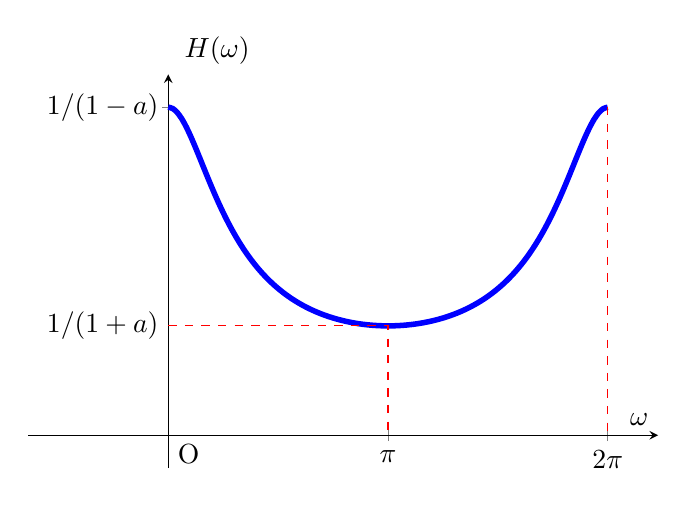
\begin{tikzpicture}
            \begin{axis}[
                axis lines = middle,
                xlabel = {$\omega$},
                ylabel = {$\abs{H(\omega)}$},
                ylabel style={at={(rel axis cs:0.3, 1)}, anchor=south},
                xmin = -2, xmax = 7,
                ymin = -0.2, ymax = 2.2,
                xtick = {0, 3.14, 6.28},
                xticklabels = {$0$, $\pi$, $2\pi$},
                ytick = {0, 2},
                yticklabels = {$ $, $ $},
                scale only axis,
                width = 8cm,
                height = 5cm,
            ]
            \addplot[domain=0:6.28, samples=100, smooth, line width=2pt, blue] {1 / sqrt(1.25 - cos(deg(x)))};
            \addplot[dashed, red] coordinates {(0, 0.667) (3.14, 0.667) (3.14, 0)};
            \addplot[dashed, red] coordinates {(6.28, 2) (6.28, 0)};
            \node at (axis cs:0, 0) [anchor=north west] {O};
            \node at (axis cs:0, 0.667) [anchor=east] {$1/(1 + a)$};
            \node at (axis cs:0, 2) [anchor=east] {$1/(1 - a)$};
            \end{axis}
        \end{tikzpicture}
        \caption{习题 \theexercise~ 的幅频响应函数}
        \label{fig:chap4-part1-quiz2-plot}
    \end{figure}
\end{solution}

\subsubsection{由差分方程求脉冲响应函数}

在性质 \ref{property:diff-equation-convolution} 中我们已经知道,
对于 FIR 系统,$h(n) = a(n)$。那么对于 IIR 系统,
\begin{align*}
    \sum_{k = 0}^{N}b(k)y(n - k) = \sum_{k = 0}^{M}a(k)x(n - k).
\end{align*}
我们应该如何求解 $h(n)$ 呢?可以考虑使用更强大的工具——Z 变换。
